%************************************************
\chapter{A Primer on Fairness Definitions} \label{ch:fairness_primer}
%************************************************

There are many mathematical definitions of fairness, each capturing different intuitive beliefs about equity. Some of the definitions of fairness turn out to be incompatible with one another in real-world scenarios. This chapter surveys common definitions of fairness and links the normative implications of each to predictive policing. Of the common notions of fairness, equalized odds is chosen as indicative of the viewpoint of an individual who cares about justice. That viewpoint will be set against the viewpoint of an individual whose main concern is accuracy in the assessment of \pp.

\section{Fairness Through Unawareness} \label{sec:fair_unaware}

One of the most popular notions of fairness, "fairness through unawareness" is the assertion that a classifier or decision-maker who does not explicitly consider protected attributes such as race and gender is fair. To explicitly consider race and gender would constitute what the United States Civil Rights Act calls "disparate treatment," and would be impermissible in many settings, such as employment \citep{barocas_big_2016}.

While intuitively satisfying to some, "fairness through unawareness" does not account for proxy discrimination. A classifier could still in practice be biased against a certain group if there is significant correlation between the protected attribute and another, seemingly innocuous variable. In the case of \pp, which does not explicitly consider race or other protected attributes in its predictions, location acts as a proxy for race (\autoref{fig:heatmaps_correlation}). The average \pp predicted intensity and percentage black has a correlation coefficient of 0.32 over 39030 grid cells (a large enough sample size to detect moderate effect sizes with statistical significance). At the same time, the correlation coefficient between the actual number of crimes committed and percentage black is only 0.11. This evidence suggests that \pp, which does not explicitly consider race, can still have different outcomes for different races (more detailed fairness analysis in \autoref{ch:results}). The point for the present discussion is that fairness through unawareness does not preclude disparate impact (also prohibited by United States civil rights law) \citep{barocas_big_2016}.

\begin{figure}[bth]
    \myfloatalign
    \subfloat[Black population as a percentage of total = black + white]
    {\label{fig:heatmap_black}%
        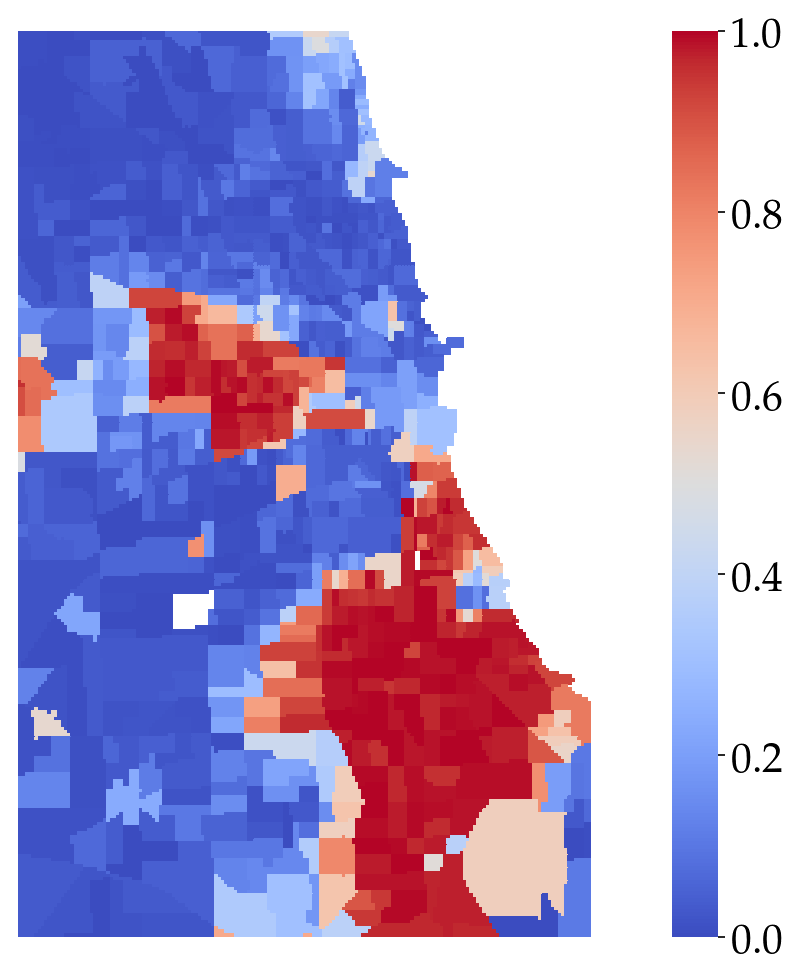
\includegraphics[height=.4\textheight]{gfx/HeatmapBlack.png}} \quad
    \subfloat[Average \pp predicted values $f$ in the year 2015]
    {\label{fig:heatmap_predicted}%
        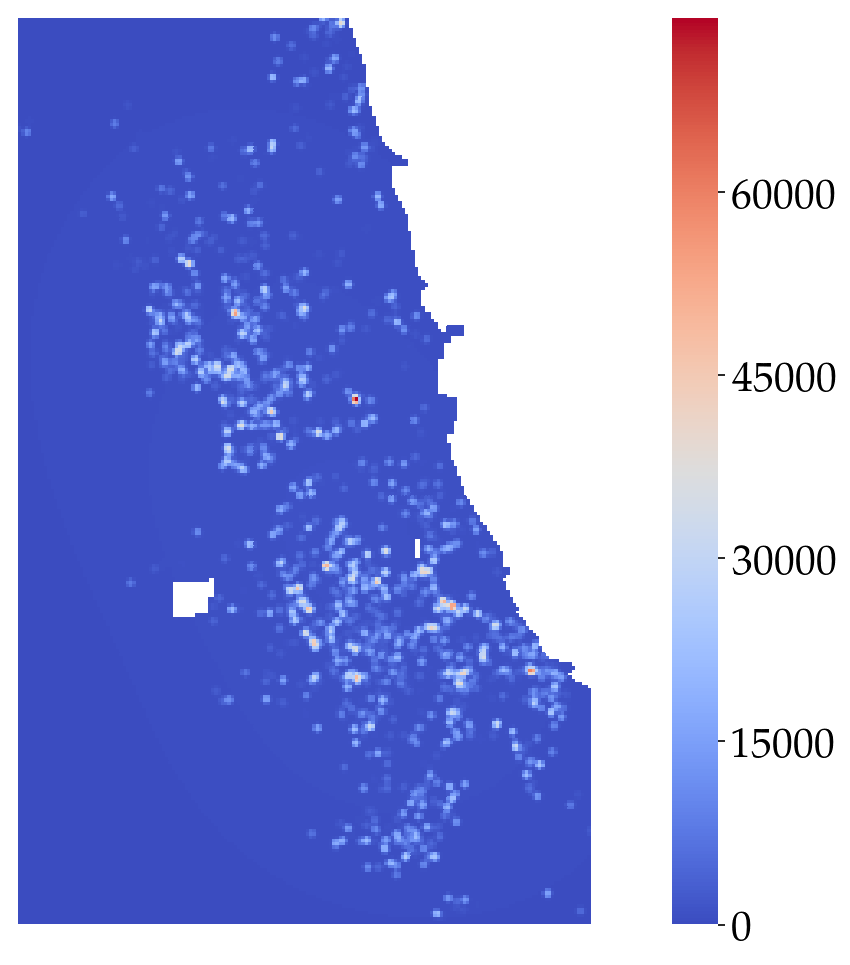
\includegraphics[height=.4\textheight]{gfx/HeatmapPredicted.png}} \\
    \caption{The visual correlation between race and \pp}
    \label{fig:heatmaps_correlation}
\end{figure}
Fairness through unawareness reflects a variety of intuitive beliefs about fairness. One intuition suggests that fairness through unawareness is the best that decision-makers or classifiers can hope for, because any other correlation between a protected attribute and the predictions might be explained as an unfortunate reflection of real-world correlation between the protected attribute and the target variable of prediction (in this case, criminality of a location). From this viewpoint, the results of \pp ought to be taken as-is, without modification. Other definitions of fairness though, attempt to take the problem of proxy discrimination seriously and control for it.

\section{Three Common Definitions}

Using conditional independence, three common definitions of fairness can be stated compactly as relationships between the ground truth $Y$, the prediction $\hat{Y}$, and the protected attribute $A$.\footnote{As a reminder of notation, the statement, "Random variable $X$ is independent of random variable $Y$ given the observation of random variable $Z$" is written as $X \perp Y \mid Z$.} Each of these definitions is observational in the sense that one does not need to conduct an intervention or run an experiment to order to assess them (causal notions of fairness do require interventions) \citep{hardt_equality_2016}. One of these definitions attempts to allow for the sort of proxy discrimination exhibited in this example up to the extent that is justified by correlation between the protected attribute and the true status. This definition also turns out to be relatively strong, insofar as it sometimes requires the decision-maker to make sacrifices to accuracy and even other notions of fairness.

The first definition, demographic parity ($\hat{Y} \perp A$), strengthens the "fairness through unawareness" condition, but ultimately to an unrealistic degree. Not only do the predictions have to be made without the protected attribute, the final predictions must also be statistically independent from the predicted attribute. This is a very stringent fairness requirement, since, as we have already seen, $Y$ and $A$ are related, and $\hat{Y}$ wants to track $Y$. Demographic parity further formalizes the notion of fairness that fairness through unawareness attempts to satisfy: in the ideal world, the true variables $Y$ are independent from protected attributes $A$. Thus, in the ideal world, either fairness through unawareness or demographic parity are sufficiently strong notions of fairness.

The next definition, equalized odds ($\hat{Y} \perp A$ | Y), can be seen as a relaxation of the previous criterion. After conditioning on the true status, the predictions ought to be independent from group status. This definition of fairness formalizes the amount of correlation that is permissible between the prediction $\hat{Y}$ and the protected group $A$: exactly as much as would be useful to predict true status.

Unlike the next and final fairness definition, which attempts to equalize accuracy across protected groups, equalized odds attempts to equalize false positive and negative rates across protected groups. The normative implications of this difference are significant, since false positives and negatives can have differing consequences on the individual and the community \citep{narayanan_21_2018}. In policing, a false positive might introduce an innocent individual into the criminal justice system, while a false negative might leave a criminal at large. In predictive policing, the individual units who are subjected to policing might be considered individual persons or the neighborhoods and locations which are recommended for patrol. If the individual units are locations, then the implication of a false positive is overpolicing a community unjustly while the implication of a false negative is underpolicing a community unduly. Equalized odds is a fairly stringent notion of fairness because satisfying it often requires sacrifices to accuracy \citep{hardt_equality_2016}.

Finally, sufficiency ($Y \perp A \mid \hat{Y}$) requires that the algorithm's overall accuracy across different groups is the same. Put differently, the location of the grid cell ought to be sufficient information for prediction and further conditioning on race (in addition to the prediction $\hat{Y}$) would not add any accuracy. This is the least stringent fairness requirement, and many out-of-the-box ML algorithms already satisfy this criterion \citep{barocas_fairness_2018}. One might intuit sufficiency in the context of predictive policing as follows: if one race is responsible for $p\%$ of the overall crime, then that race ought to be policed $p\%$ of the time.\footnote{Out of the box, \pp does not appear to satisfy this definition of fairness (\autoref{sec:sufficiency}). The upshot is that the predicted intensities from \pp have different interpretations based on the demographic makeup of the grid cell, a line of inquiry which is not pursued in this research.}

Sufficiency and equalized odds are incompatible whenever the baseline rate of true status differs between groups \citep{kleinberg_inherent_2016,chouldechova_fair_2017}.\footnote{\autoref{proof:ch_3} offers an alternative proof of this incompatibility using the $p\%$ intuition for sufficiency suggested above.} In the real-world, one can usually only ask that either sufficiency or equalized odds are met.

We will assess \pp on and make \pp fairer with respect to equalized odds because equalized odds is a stronger notion of fairness than sufficiency without being obviously deficient like demographic parity. Sufficiency is too weak a notion of fairness because it ignores the consequential difference between false positives and negatives in many contexts. Some have argued though, that because of the impossibility of achieving both  equalized odds and sufficiency, one ought to focus on deploying predictors which are as accurate as possible while also ensuring that the processes around the predictor are also just \citep{corbett-davies_algorithmic_2017}. Essentially, this view bites the bullet on the impossibility theorem, and accepts the fact that equalized odds will not be met in many real-world scenario. Where there is some merit to this view, especially since observational notions of fairness themselves do not guarantee that algorithms are used justly, there are probably still scenarios in which having an equalized odds predictor would be useful. Moreover, the aim of this thesis is to show how \pp fails to impress either on accuracy or on a relatively stringent notion of fairness. We do not claim to have the final word on all normative concerns surrounding algorithmic fairness.
% Since \pp by default satisfies sufficiency, equalized odds will be the target metric of fairness for the present research. However, that does not discount the viewpoint of sufficiency (or fairness through unawareness). This paper takes both the perspective of no fairness constraints---accuracy is the only important criterion---and of relatively strong fairness constraints. We will show how \pp, scored on either accuracy or equality of opportunity, fails to impress.

Finally, as a cautionary note regarding the usage of technical notions of fairness, ensuring equalized odds in predictions does not guarantee the equal distribution of risk or burden in reality. For example, in the context of predictive policing, individuals may still face heightened scrutiny for their racial features, regardless of which grid cells \pp ultimately predicts. The task of equalizing burden in practice requires, as \citet{perry_predictive_2013} suggested, best practices throughout the whole policing pipeline.
